\subsection{Лабораторная работа № 3}

\subsubsection{Задача}

Создать двух пользователей базы данных, обладающих различными правами доступа.
Первый пользователь должен быть предназначен для просмотра статистики по
начертаниям. Второй пользователь должен иметь возможность работать с
агрегированными и исходными данными, связанными с этой статистикой.

\begin{enumerate}
    \item Пользователь \mintinline{text}{stats_reader} может только
    просматривать таблицу
    \mintinline{text}{typeface_format_weight_stats}. Ему доступна операция
    \mintinline{sql}{SELECT} из этой таблицы, ко всем остальным таблицам
    доступа нет.
    \item Пользователь \mintinline{text}{source_editor} имеет полный доступ
    к таблицам \mintinline{text}{Font_family} и
    \mintinline{text}{Typeface}, изменения которых влияют на таблицу
    статистики. Ему также разрешено чтение и изменение
    \mintinline{text}{typeface_format_weight_stats}. Доступ к остальным
    таблицам базы данных запрещён.
\end{enumerate}

Для проверки назначенных прав требуется выполнить один набор тестовых запросов
от имени обоих пользователей и сопоставить полученные результаты.

\subsubsection{Создание пользователей и назначение прав}

Командами \mintinline{sql}{CREATE USER} создаются
пользователи \mintinline{text}{stats_reader} и
\mintinline{text}{source_editor}. Обоим пользователям разрешаются подключение
к базе данных, использование схемы \mintinline{text}{public} и чтение таблицы
статистики. Пользователь \mintinline{text}{source_editor} дополнительно
получает права на изменение связанных таблиц и используемые ими
последовательности. Полный скрипт приведён в
листинге~\ref{lst:pr-03-users}.

\codeListing[sql]
{../practice-03/src/users.sql}
{Создание пользователей и назначение прав}
{\label{lst:pr-03-users}}

\subsubsection{Тестовые примеры}

Для проверки прав подготовлено десять запросов. Каждый запрос выполняется без
изменений сначала от имени \mintinline{text}{stats_reader}, затем от имени
\mintinline{text}{source_editor}.

Первый запрос проверяет чтение таблицы статистики. Эта операция должна быть
доступна обоим пользователям. Текст запроса приведён в
листинге~\ref{lst:pr-03-query-01}.

\codeListing[sql]{../practice-03/tests/queries/01-select-stats.sql}
{Чтение таблицы статистики}
{\label{lst:pr-03-query-01}}

Второй запрос проверяет возможность непосредственного добавления строки
таблицы статистики. Третий запрос читает её по составному первичному ключу,
а четвёртый удаляет. Тексты запросов приведены в
листингах~\ref{lst:pr-03-query-02}--\ref{lst:pr-03-query-04}.

\codeListing[sql]{../practice-03/tests/queries/02-insert-stats.sql}
{Добавление строки таблицы статистики}
{\label{lst:pr-03-query-02}}

\codeListing[sql]{../practice-03/tests/queries/03-select-inserted-stats.sql}
{Проверка добавленной строки таблицы статистики}
{\label{lst:pr-03-query-03}}

\codeListing[sql]{../practice-03/tests/queries/04-delete-stats.sql}
{Удаление строки таблицы статистики}
{\label{lst:pr-03-query-04}}

Пятый запрос добавляет тестовое начертание, копируя значения внешних
ключей из первой существующей строки. Текст запроса приведён в
листинге~\ref{lst:pr-03-query-05}.

\codeListing[sql]{../practice-03/tests/queries/05-insert-typeface.sql}
{Добавление тестового начертания}
{\label{lst:pr-03-query-05}}

Шестой запрос проверяет наличие добавленного начертания в исходной таблице
\mintinline{text}{Typeface}. Седьмой запрос изменяет его название, а восьмой
выбирает изменённую строку по идентификатору. Тексты запросов приведены в
листингах~\ref{lst:pr-03-query-06}--\ref{lst:pr-03-query-08}.

\codeListing[sql]{../practice-03/tests/queries/06-select-typeface.sql}
{Проверка добавленного начертания}
{\label{lst:pr-03-query-06}}

\codeListing[sql]{../practice-03/tests/queries/07-update-typeface.sql}
{Изменение тестового начертания}
{\label{lst:pr-03-query-07}}

\codeListing[sql]{../practice-03/tests/queries/08-select-updated-typeface.sql}
{Проверка изменённого начертания}
{\label{lst:pr-03-query-08}}

Девятый запрос обращается к таблице \mintinline{text}{Category}, права на
которую не были назначены ни одному из пользователей. Десятый запрос удаляет
добавленное ранее тестовое начертание. Тексты запросов приведены в
листингах~\ref{lst:pr-03-query-09} и~\ref{lst:pr-03-query-10}.

\codeListing[sql]{../practice-03/tests/queries/09-select-category.sql}
{Чтение таблицы без назначенных прав}
{\label{lst:pr-03-query-09}}

\codeListing[sql]{../practice-03/tests/queries/10-delete-typeface.sql}
{Удаление тестового начертания}
{\label{lst:pr-03-query-10}}

\subsubsection{Результаты тестирования}

Результаты выполнения одного набора запросов от имени двух пользователей
сопоставлены в таблице~\ref{table:pr-03-access-tests}. В первой строке каждого
примера приведён текст запроса, во второй --- результаты его выполнения.

\begin{aThreePortraitPage}

\newcommand{\queryCell}[1]{%
    \begin{minipage}{0.9\textwidth}
        \raggedright\small\ttfamily #1
    \end{minipage}%
}

\begin{table}[H]
\centering
\caption{Результаты тестовых запросов}
\label{table:pr-03-access-tests}
\begin{tblr}{
    width=\textwidth,
    colspec={Q[c,2.2em]X[l]X[l]},
    hlines,
    vlines,
    row{1}={font=\bfseries},
    rows={valign=m},
    cell{2-Z}{2-Z}={preto=\small},
}
    № & \mintinline{text}{stats_reader} &
    \mintinline{text}{source_editor} \\

    \SetCell[r=2]{c} 1 &
    \SetCell[c=2]{l} \queryCell{SELECT * FROM typeface\_format\_weight\_stats LIMIT 3;} & \\
    & \SetCell[c=2]{c}
    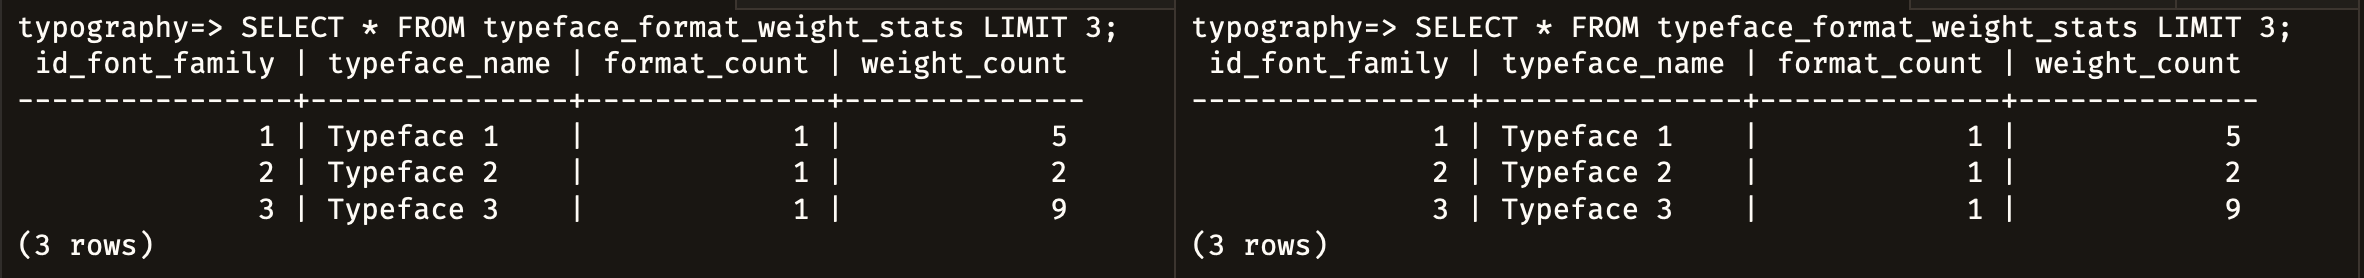
\includegraphics[width=0.95\textwidth]{img/pr-03-query-01-result.png} & \\

    \SetCell[r=2]{c} 2 &
    \SetCell[c=2]{l} \queryCell{INSERT INTO typeface\_format\_weight\_stats (...) VALUES (-1, 'Permission test', 1, 1);} & \\
    & \SetCell[c=2]{c}
    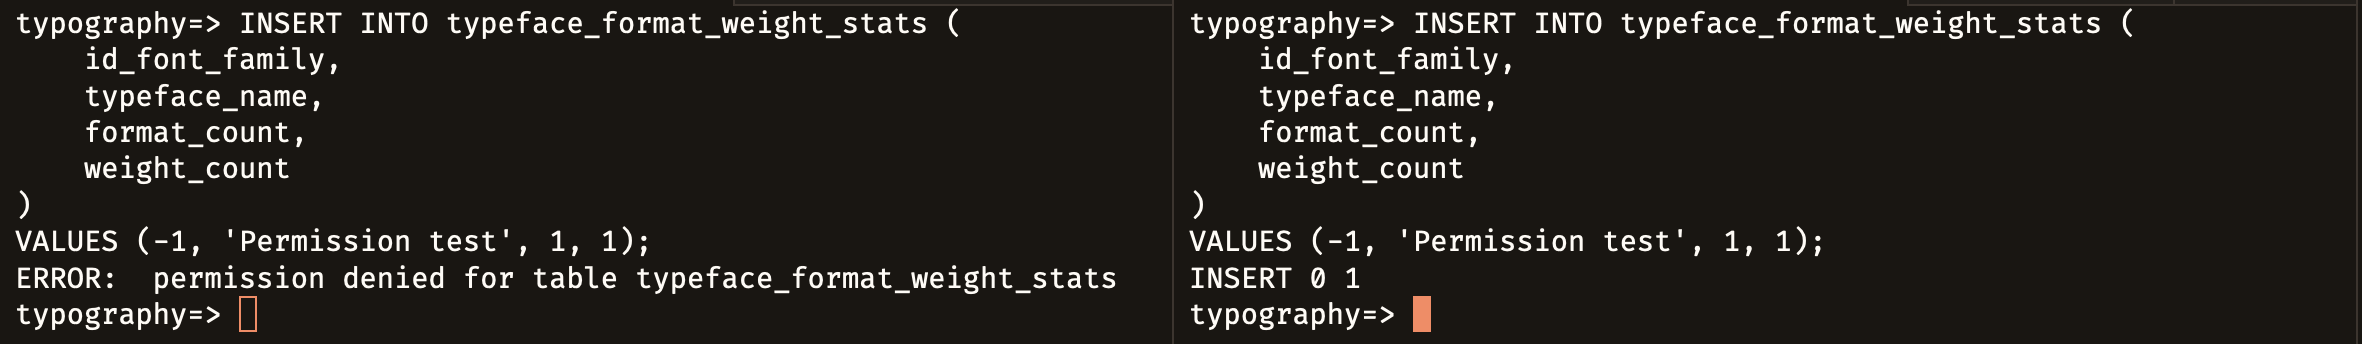
\includegraphics[width=0.95\textwidth]{img/pr-03-query-02-result.png} & \\

    \SetCell[r=2]{c} 3 &
    \SetCell[c=2]{l} \queryCell{SELECT * FROM typeface\_format\_weight\_stats WHERE id\_font\_family = -1 AND typeface\_name = 'Permission test';} & \\
    & \SetCell[c=2]{c} \rule{0pt}{18mm} & \\

    \SetCell[r=2]{c} 4 &
    \SetCell[c=2]{l} \queryCell{DELETE FROM typeface\_format\_weight\_stats WHERE id\_font\_family = -1;} & \\
    & \SetCell[c=2]{c}
    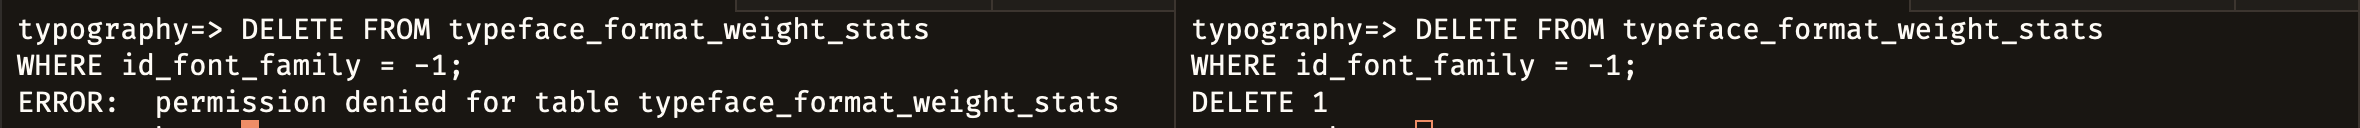
\includegraphics[width=0.95\textwidth]{img/pr-03-query-04-result.png} & \\

    \SetCell[r=2]{c} 5 &
    \SetCell[c=2]{l} \queryCell{INSERT INTO typeface (...) SELECT ... FROM typeface ORDER BY id\_typeface LIMIT 1;} & \\
    & \SetCell[c=2]{c}
    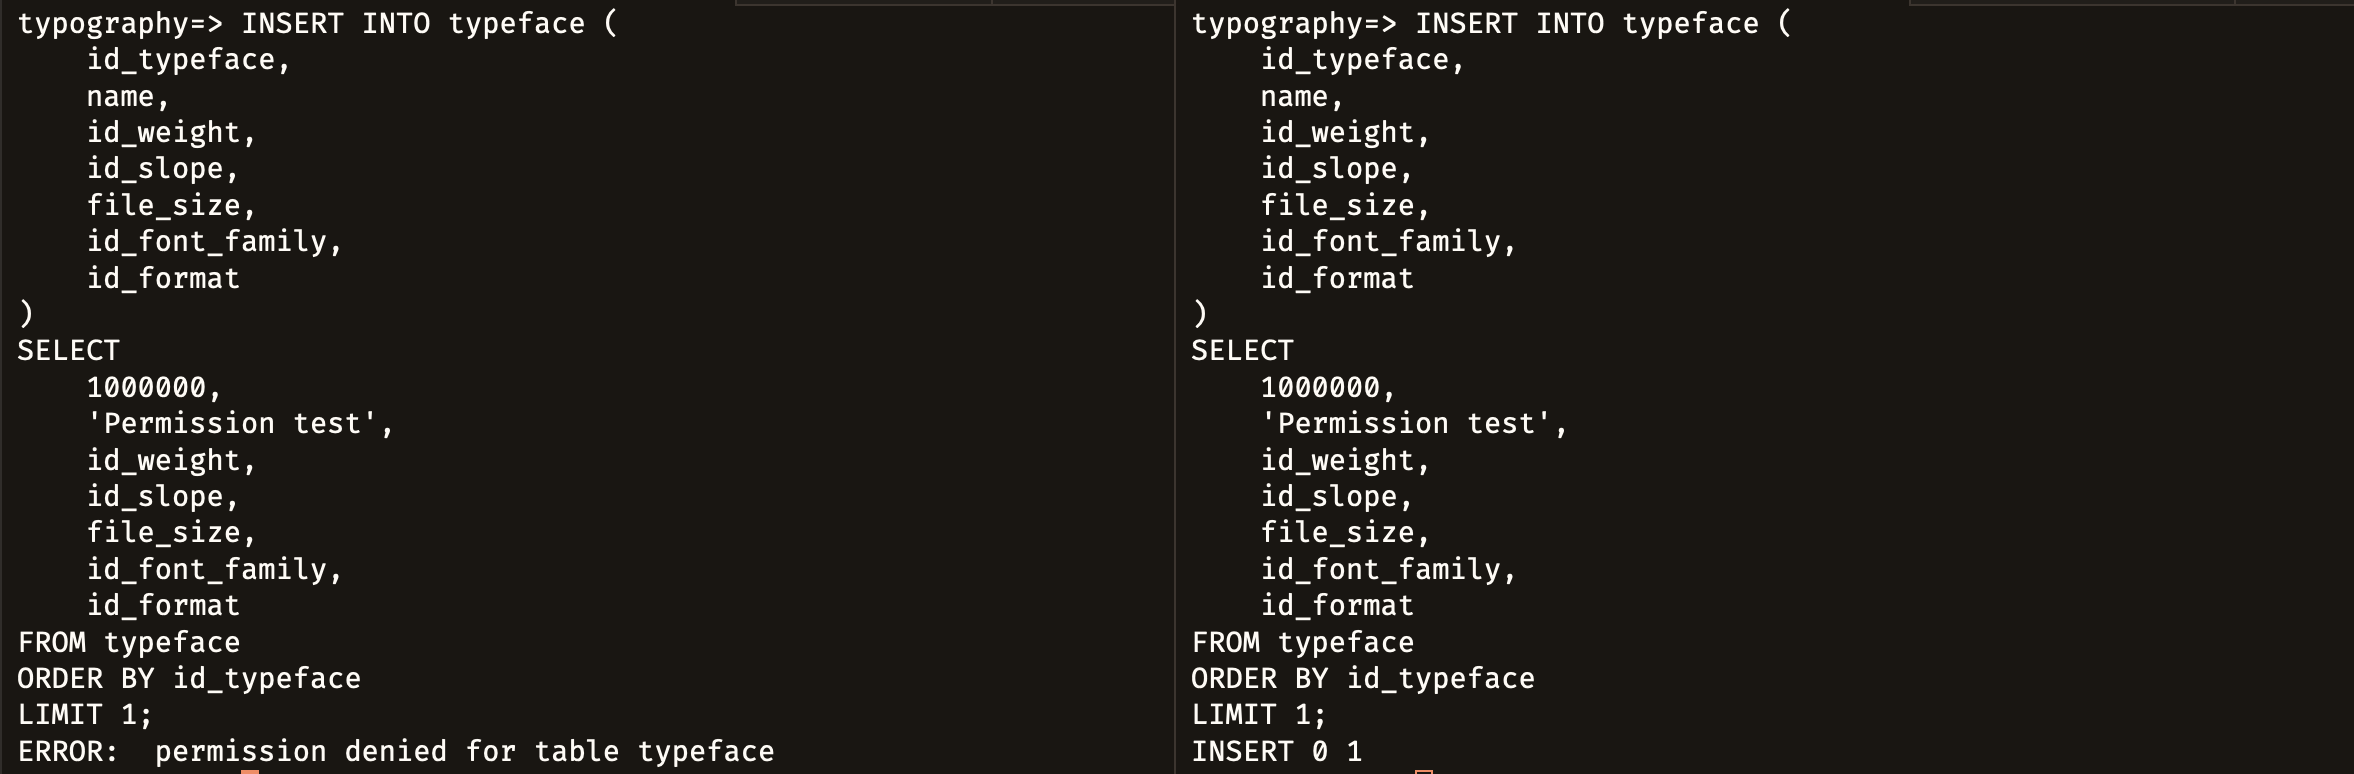
\includegraphics[width=0.95\textwidth]{img/pr-03-query-05-result.png} & \\

    \SetCell[r=2]{c} 6 &
    \SetCell[c=2]{l} \queryCell{SELECT id\_typeface, name FROM typeface WHERE name = 'Permission test';} & \\
    & \SetCell[c=2]{c}
    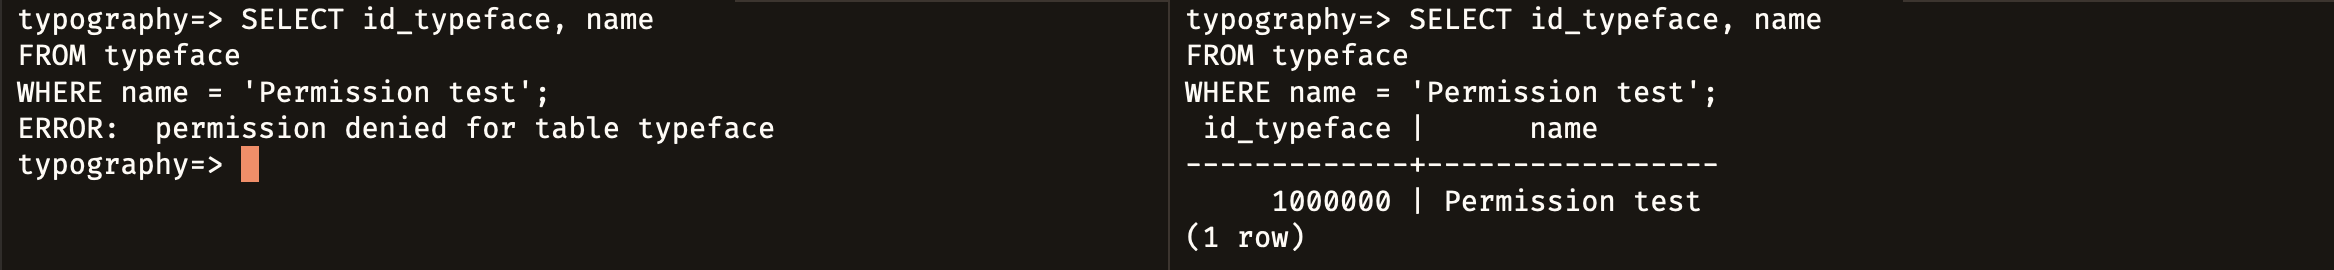
\includegraphics[width=0.95\textwidth]{img/pr-03-query-06-result.png} & \\

    \SetCell[r=2]{c} 7 &
    \SetCell[c=2]{l} \queryCell{UPDATE typeface SET name = 'Permission test updated' WHERE id\_typeface = 1000000;} & \\
    & \SetCell[c=2]{c}
    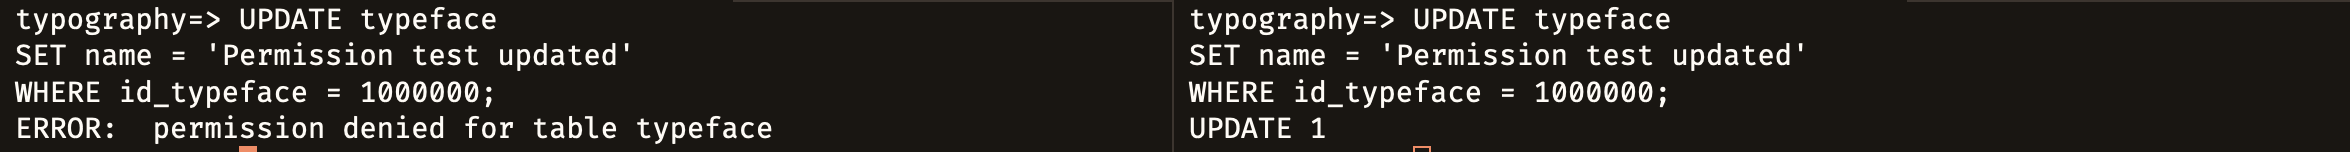
\includegraphics[width=0.95\textwidth]{img/pr-03-query-07-result.png} & \\

    \SetCell[r=2]{c} 8 &
    \SetCell[c=2]{l} \queryCell{SELECT id\_typeface, name FROM typeface WHERE id\_typeface = 1000000;} & \\
    & \SetCell[c=2]{c} \rule{0pt}{18mm} & \\

    \SetCell[r=2]{c} 9 &
    \SetCell[c=2]{l} \queryCell{SELECT * FROM category LIMIT 3;} & \\
    & \SetCell[c=2]{c}
    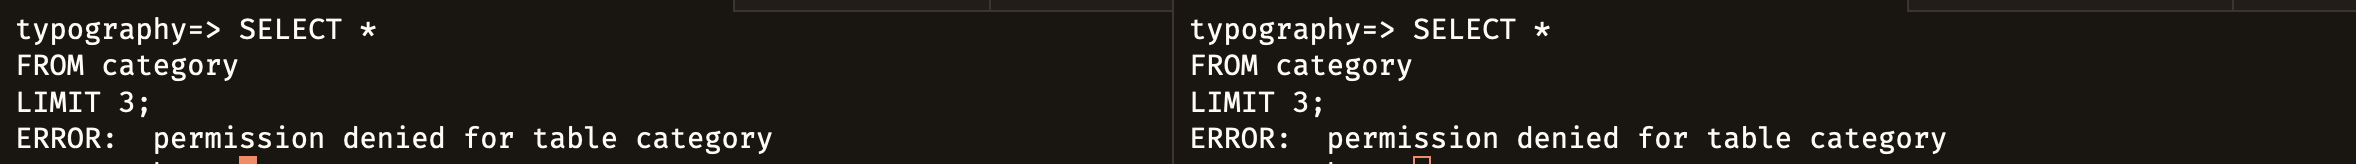
\includegraphics[width=0.95\textwidth]{img/pr-03-query-09-result.png} & \\

    \SetCell[r=2]{c} 10 &
    \SetCell[c=2]{l} \queryCell{DELETE FROM typeface WHERE id\_typeface = 1000000;} & \\
    & \SetCell[c=2]{c}
    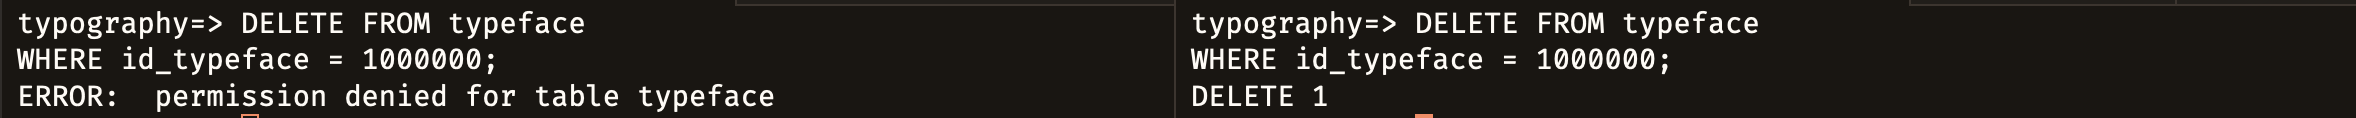
\includegraphics[width=0.95\textwidth]{img/pr-03-query-10-result.png} & \\
\end{tblr}
\end{table}

\end{aThreePortraitPage}
